\documentclass{jlreq}

\usepackage{amsmath}
\usepackage{bm}
\usepackage{fancyhdr}
\usepackage{float}
\usepackage{graphicx}
\usepackage{physics}
\usepackage{siunitx}

\numberwithin{equation}{section}

\pagestyle{fancy}
\fancyhf{}
\fancyhead[R]{\thepage}

\begin{document}

\tableofcontents
\clearpage

\section{実験項目}
% ここに項目を記入

\section{目的}
\subsection{2週目}
LCR回路のインディシャル応答を調べ,時間応答特性について検討する.

\subsection{3週目}
LCR回路のゲイン特性と位相特性のデータをもとにボード線図を作成する.

\section{使用するソフトと部品}
\begin{itemize}
  \item Excel
  \item LCR電子回路コンポネント
  \item ブレッドボード
  \item Analog Discovery
  \item WaveForms
\end{itemize}

\section{結果}
LCR回路の部品は表\ref{tab:lcr_components}の値を用いた.また,オペアンプは用いていない.
\begin{table}[H]
  \centering
  \caption{用いたLCR回路の部品}
  \begin{tabular}{|c|c|c|}
    \hline
    抵抗(\si{\Omega}) & コンデンサ(\si{\micro\farad}) & コイル(\si{\milli\henry}) \\ \hline
    33                & 2.2                           & 30                        \\ \hline
  \end{tabular}
  \label{tab:lcr_components}
\end{table}

表\ref{tab:lcr_components}の部品を用いたLCR回路のインディシャル応答の理論値と実測値は図\ref{fig:lcr_indicial_without_opamp}のようになった.
\begin{figure}[H]
  \centering
  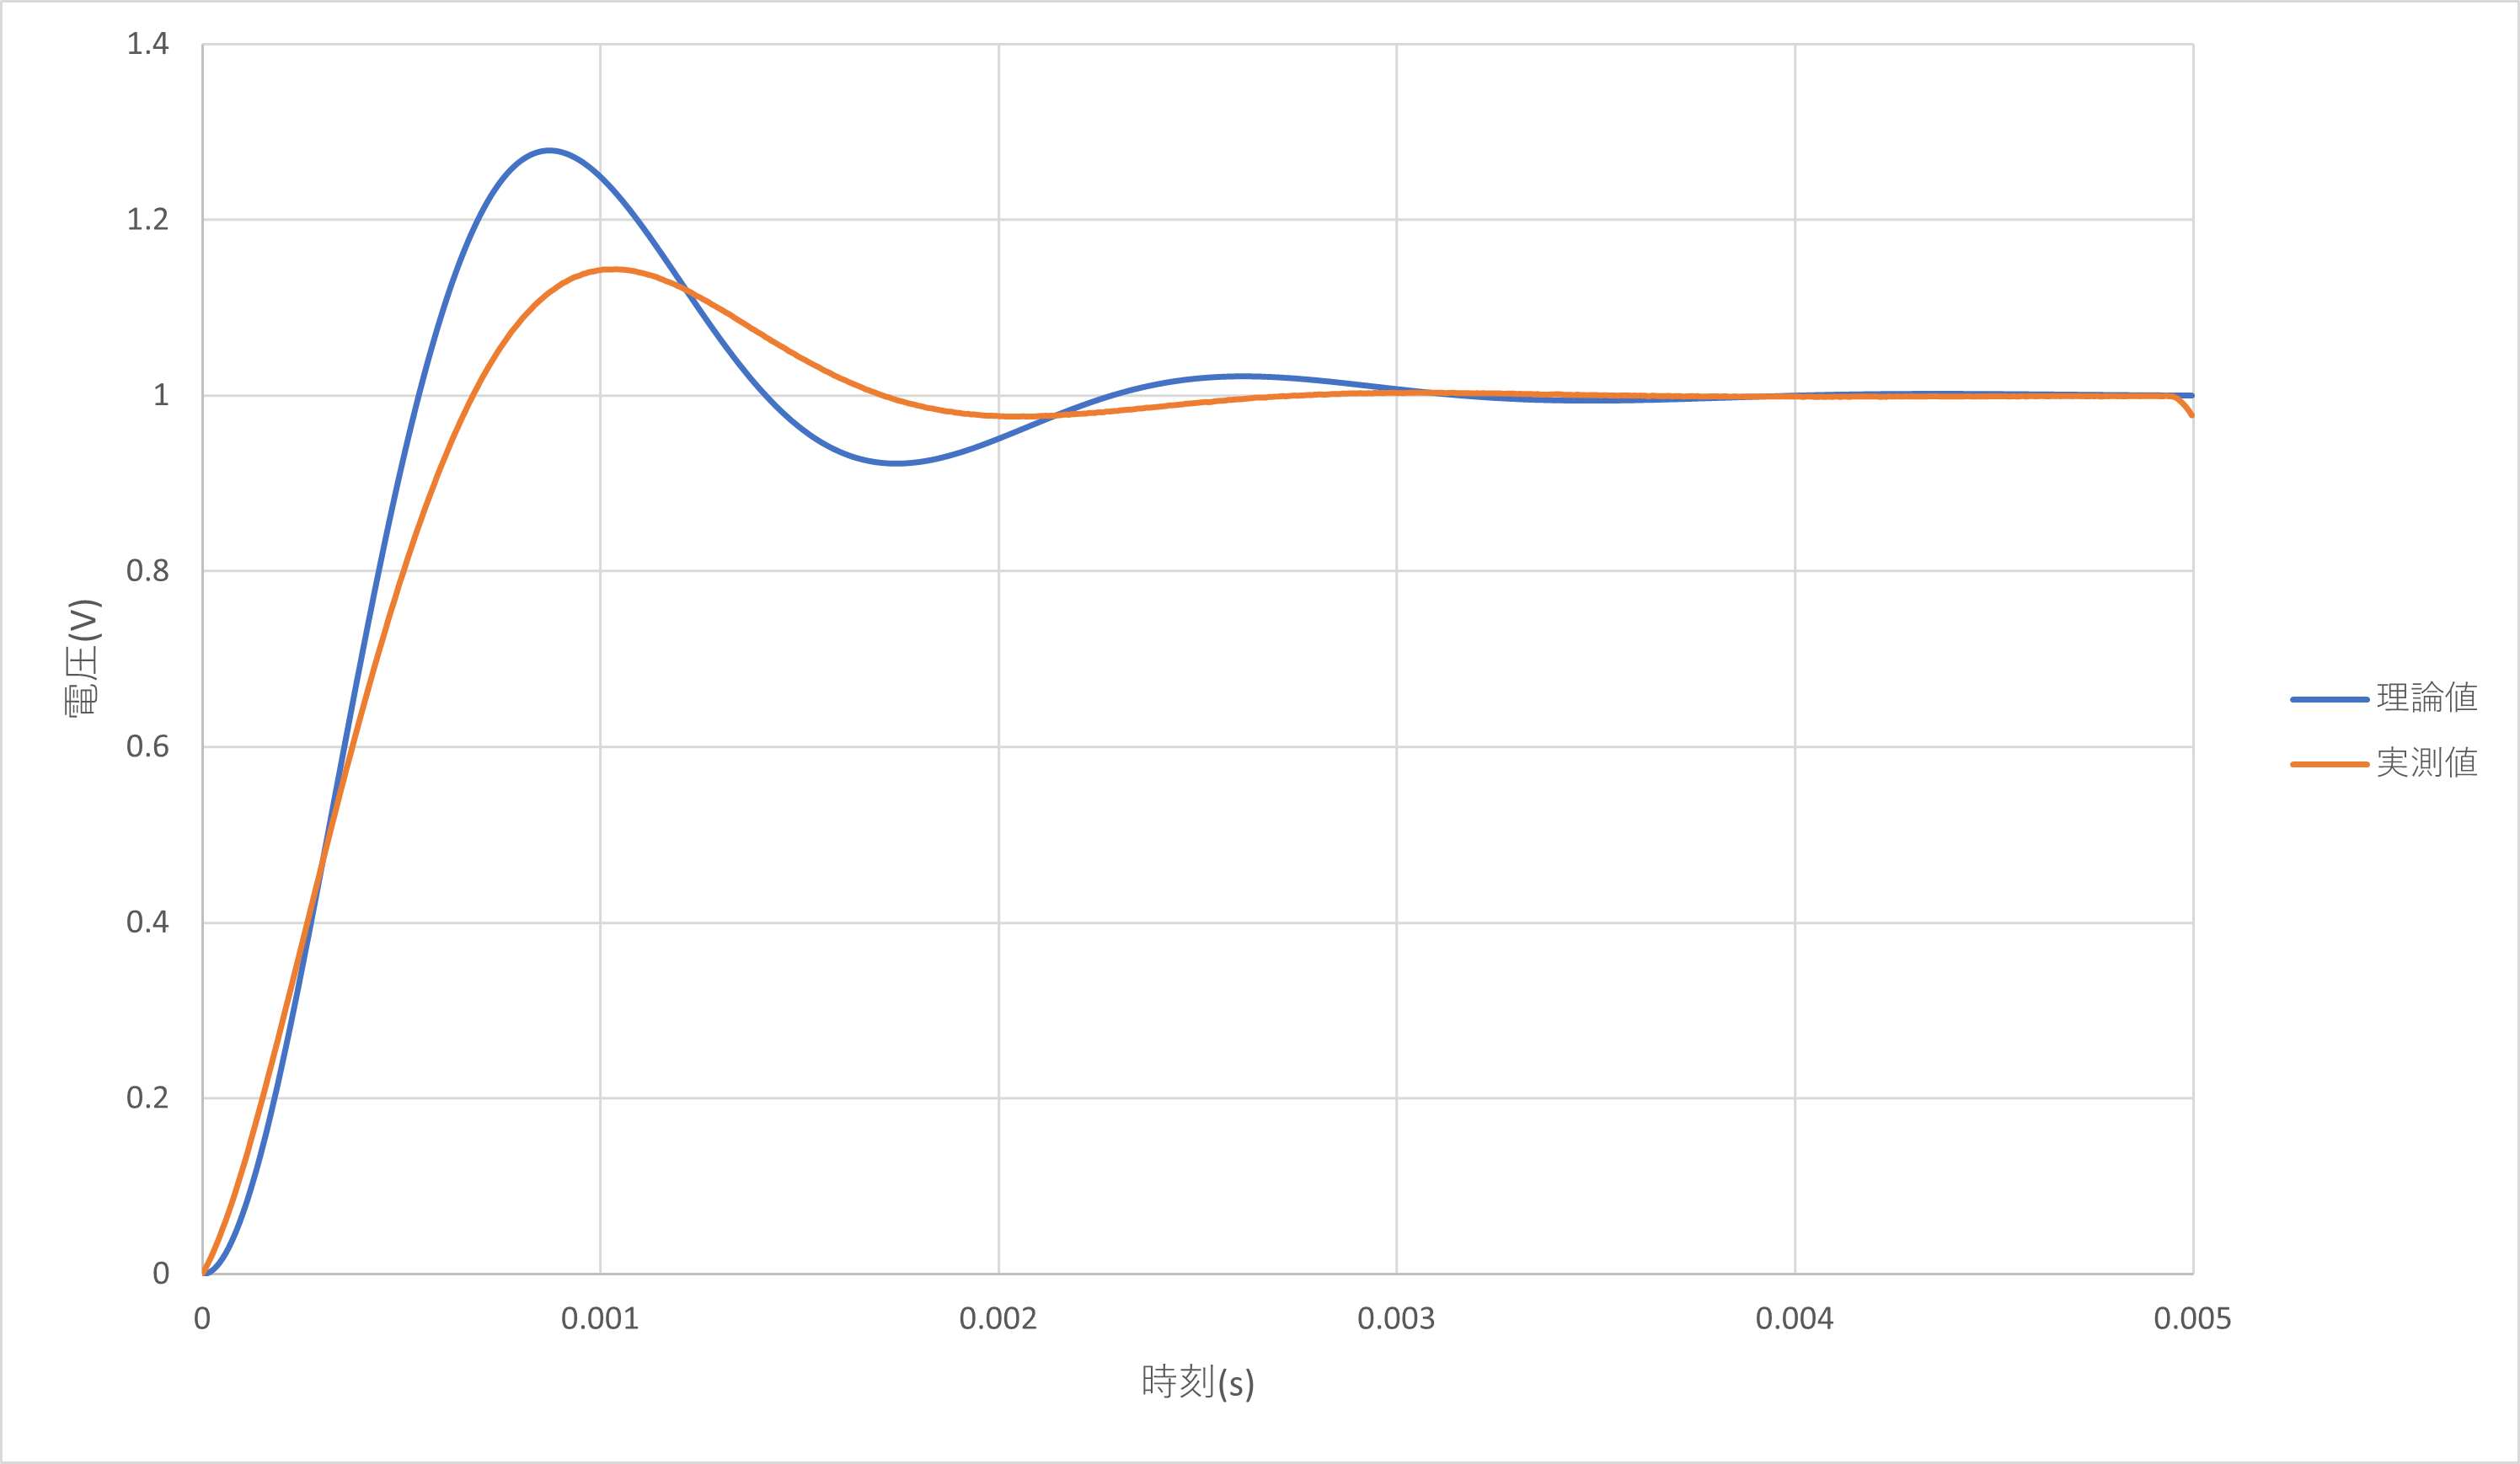
\includegraphics[width=\textwidth]{assets/lcr_indicial_without_opamp.png}
  \caption{LCR回路のインディシャル応答の比較図}
  \label{fig:lcr_indicial_without_opamp}
\end{figure}

\section{考察}
\subsection{インディシャル応答の測定値と実測値の比較}
図\ref{fig:lcr_indicial_without_opamp}から,理論値に比べて実測値は電圧の最大値が低く,一定に落ち着くまでの曲線の振動が少なくなだらかである.
これは,実際に用いた部品の抵抗値が錆などによって高くなっており,曲線の揺れ方に影響したのではないかと考えられる.

\subsection{}

\section{問題の解答}
\subsection*{課題4.5.1}
実験テキストのボード線図を確認すると,比較的低い周波数の正弦波を入力としたときにはゲインが$0 \si{\decibel}$で一定となっており,これは入出力で振幅に変化が見られないことを意味する.
また位相に関しても,周波数が比較的低い場合は$0 \si{\degree}$近辺のなだらかな曲線となっており,入出力で位相のずれが小さいと考えられる.

\subsection*{課題4.5.2}
実験テキストのボード線図を確認すると,比較的高い周波数の正弦波を入力としたときにはゲインが負の方向に発散しており,入力に対する出力の振幅がますます小さくなることを意味する.
また位相に関しても,周波数が比較的高い場合は$-90 \si{\degree}$に限りなく近くなるため,入力に対する出力の位相はほぼ$-90 \si{\degree}$となる.

\begin{thebibliography}{9}
  \item シリアーラヤ パノット.プロジェクト実習Ⅰ エレクトロニクス基礎 実験テキスト.京都工芸繊維大学,2024年
\end{thebibliography}

\end{document}